\chapter{Introduction \& Background}
\label{sec:introduction-background}
\newpage

The contemporary digital landscape has fundamentally transformed how information is distributed and consumed. The transition from traditional print and scheduled broadcast media to real-time digital syndication has compressed the news lifecycle, enabling instantaneous updates but simultaneously accelerating the propagation of unverified claims, polarized narratives, and coordinated misinformation. processing this massive volume of high-velocity textual data in real-time presents a severe challenge for standard media analysis systems. Manual fact-checking pipelines cannot scale to handle this throughput, while conventional automated solutions rely on massive, monolithic artificial intelligence models that introduce prohibitive operational costs and high inference latency.

This chapter introduces NewsPulse, a highly decoupled, microservices-based intelligence platform engineered to aggregate, summarize, and analyze news articles along multiple dimensions. Designed to operate within strictly constrained local hardware environments, NewsPulse circumvents the need for expensive, GPU-accelerated cloud architectures and proprietary generative model APIs. By utilizing highly optimized, CPU-friendly HuggingFace Transformers, PyTorch dynamic integer quantization, and robust deterministic natural language processing fallbacks, the system executes sub-second multi-dimensional analysis on consumer-grade central processing units. The platform coordinates these stateless analytic engines behind an API gateway secured with end-to-end payload encryption, exposing operational insights via local telemetry tools.

\section{Background}
Automated computational journalism has traditionally depended on centralized, monolithic architectures to collect, classify, and distribute digital news. These monolithic systems struggle with scalability when subjected to modern concurrent traffic loads, as a performance bottleneck in one pipeline component (such as model loading or tokenization) can degrade the entire application's availability. Furthermore, the modern news ecosystem is heavily saturated with sensationalist styling and politically polarized framing, which standard statistical text classifiers frequently misinterpret.

To address these vulnerabilities, modern software engineering favors the decomposition of complex platforms into isolated, stateless microservices. When combined with local machine learning models, this microservices paradigm allows specialized containers to scale independently based on their specific CPU or memory usage. To ensure the trustworthiness of the automated metrics, these models must provide explainable visual feedback (Explainable Artificial Intelligence or XAI) rather than returning opaque scalar indicators. In resource-constrained deployment environments lacking dedicated hardware accelerators (such as graphics processing units or tensor processing units), this microservice topology must be fortified with deterministic, low-overhead fallback heuristics to maintain continuous availability under heavy system load.

\section{Motivation and Challenges}
The core engineering challenge addressed by this project is the construction and deployment of a multi-service NLP pipeline within severe local hardware restrictions, specifically targeting consumer-grade CPUs with restricted random-access memory. 

The primary technical challenges include:
\begin{itemize}
    \item \textbf{Resource Exhaustion and Tensor Overflows:} Large-scale transformer models easily saturate system memory when processing long-form journalism. When tokenizing articles exceeding standard sequence boundaries, traditional encoder-decoder pipelines can suffer from tensor indexing errors and out-of-memory crashes. NewsPulse addresses this constraint by implementing character-level hard truncation limits (e.g., capping summarizer inputs at 2500 characters) and processing long texts through overlapping 512-token sliding window arrays to ensure safe and stable execution.
    \item \textbf{Data Heterogeneity and Network Blocking:} Digital news feeds frequently supply incomplete payloads or truncated description snippets. Furthermore, standard scraping tools often trigger security blocks, TLS handshake timeouts, and anti-bot defenses. To bypass these limitations, this project designs a resilient, multi-tiered crawler that sequentially falls back from an async HTTP client with randomized user-agent spoofing to a native scraping engine, and ultimately to an unverified TLS connection bypassing certificate checks.
    \item \textbf{Explainability Deficits in Black-Box Models:} Standard deep-learning classification models function as mathematical black boxes, outputting bias or credibility scores without explaining the specific linguistic triggers. This lack of transparency prevents users from critically evaluating the system's conclusions. The system resolves this challenge by computing localized, sentence-level stylometric sensationalism metrics and identifying highly biased token sequences to highlight specific triggering sentences for the end-user.
    \item \textbf{Payload Transit Vulnerability:} Transmitting sensitive user preferences, reading histories, and raw analytics requests in cleartext exposes the system to traffic interception and profiling. To protect user data privacy without introducing significant latency, the architecture integrates a robust hybrid cryptosystem that handles asymmetric and symmetric encryption directly between the client interface and the gateway service.
\end{itemize}

\section{Goals and Objectives}
The primary objective of the NewsPulse system is to build a highly optimized, local intelligence engine that delivers real-time news collection and multi-dimensional analysis. The functional objectives of the platform are defined as follows:

\begin{enumerate}
    \item \textbf{Asynchronous Multi-Source Aggregation:} Engineer a localized background daemon utilizing asynchronous event loops to poll news APIs and RSS feeds every 15 minutes. The engine must clean the scraped HTML, classify the articles into distinct categories using keyword heuristics, deduplicate the stories using fast string normalization, and cache the processed array in Redis to serve as a zero-latency landing feed.
    \item \textbf{Hardware-Optimized Summarization:} Implement an abstractive summarization service using a local DistilBART model. To prevent resource saturation, the service must enforce character-level input limits. If the deep-learning model fails or system memory is depleted, the service must seamlessly fall back to a deterministic extractive algorithm that scores sentences based on term frequency with a square-root sentence length penalty.
    \item \textbf{Multi-Signal Consensus Credibility Assessment:} Deploy a consensus architecture (the Sentinel engine) that determines credibility by combining five distinct signals: localized BERT classification, custom stylometric density analysis (sensational vocabulary, capitalization ratios, exclamation densities, and clickbait patterns), cognitive complexity metrics (lexical diversity and subjectivity ratios), domain credibility scales, and live fact-check verification queries.
    \item \textbf{Context-Aware Bias Detection:} Develop an analytical service to estimate political polarization using a DistilRoBERTa model trained on news bias datasets. The model must process articles via overlapping 512-token windows and compute a weighted average of chunk probabilities, emphasizing the introduction and conclusion segments. The service must integrate an apolitical topic gate to suppress false-positive bias scores on sports, technology, and science journalism.
    \item \textbf{Quantized Socratic Debater Engine:} Construct a counter-argument generator powered by a quantized sequence-to-sequence model (LaMini-Flan-T5) optimized via PyTorch Dynamic INT8 Quantization. The system must post-process the generated text to eliminate model loop repetitions and grammatical errors, and fall back to a deterministic rule-based template engine that extracts proper nouns and matches domains if resources are exhausted.
    \item \textbf{Secure Cryptographic Transit:} Enforce comprehensive payload security using a hybrid cryptosystem. All communications between the client interface and the API gateway must be protected by encrypting payloads using AES-256-GCM, with the symmetric keys securely exchanged using RSA-2048 (OAEP-SHA256) standards.
\end{enumerate}

\section{Literature Review/Existing Solutions}
Recent research in automated news processing favors massive generative models hosted in cloud environments. While these models are highly capable, they introduce significant network latency, require substantial operational budgets, and expose sensitive user data to third-party providers. 

 bias detection systems documented in contemporary literature often utilize rigid, global token-classification matrices. Because these matrices do not account for domain-specific context, they frequently misclassify objective technical terms or highly descriptive sports commentary as politically biased. Furthermore, standard fact-checking and fake news detection applications rely on single-model predictions. By ignoring secondary stylometric markers, lexical diversity, or publisher track records, these applications remain highly vulnerable to adversarial text alterations and model hallucinations.

\section{Gap Analysis}
A rigorous evaluation of current news aggregation and analysis applications highlights three critical technological gaps:
\begin{itemize}
    \item \textbf{Unified Multi-Signal Classification:} Existing platforms separate aggregation, summarization, credibility evaluation, and bias detection into independent applications. No localized platform combines these processes into a unified analytical suite capable of running on standard hardware.
    \item \textbf{Explainable AI in News Analysis:} Modern analytics tools typically output binary classifications or scalar confidence scores without identifying the underlying textual evidence. The absence of sentence-level highlighting prevents users from understanding *why* a particular piece of journalism was flagged as biased or sensationalist.
    \item \textbf{System Telemetry and decoupling:} Most open-source news tools are built as monolithic applications that lack integrated performance monitoring. This makes it difficult to track system bottlenecks or model latency under concurrent load.
\end{itemize}

NewsPulse addresses these deficiencies by establishing a modular microservice architecture that isolates each analytical engine, implements sentence-level XAI highlighting, and integrates real-time telemetry tracking.

\section{Proposed Solution}
The proposed system is structured as an 11-container Dockerized ecosystem designed to decouple data ingestion, cryptographic security, stateful storage, and machine learning inference. 

\begin{figure}[h]
\centering
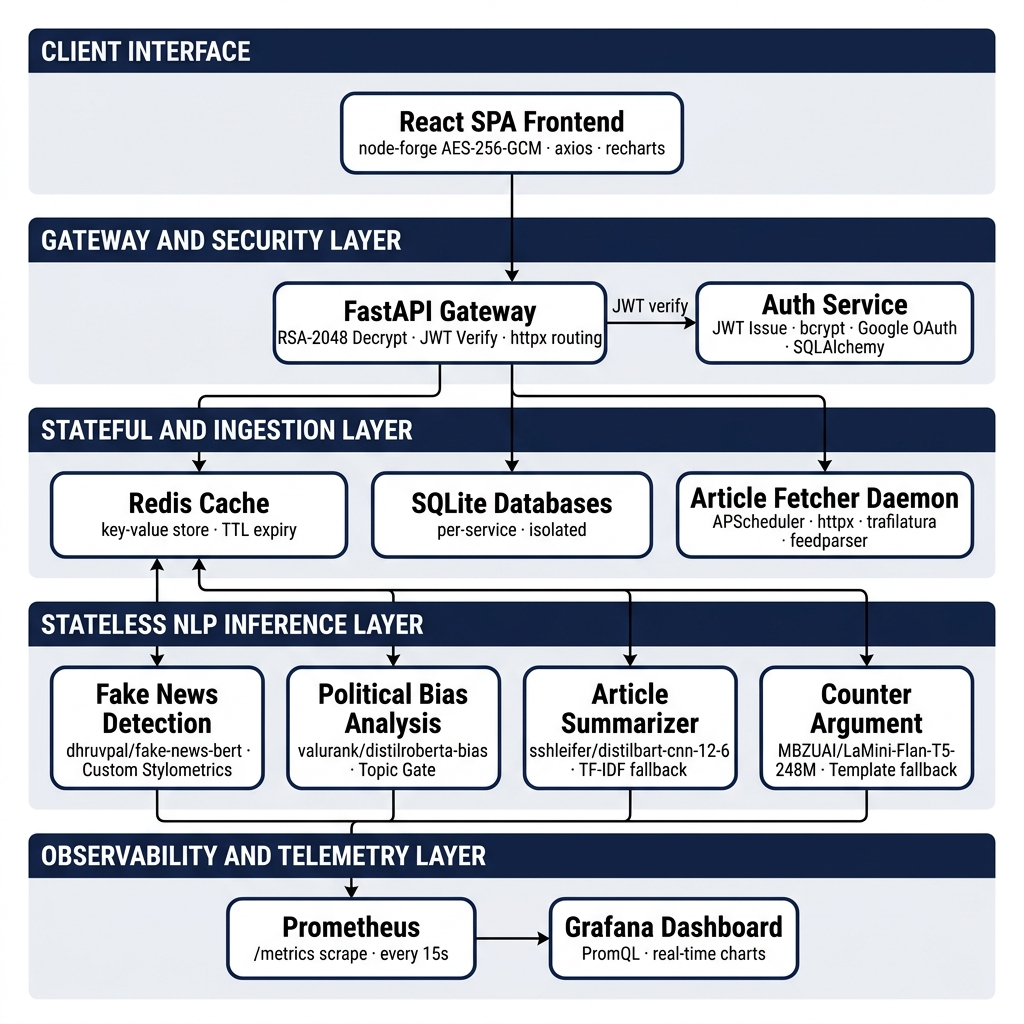
\includegraphics[width=\textwidth]{BS_FYP_Figs/system_architecture.png}
\caption{NewsPulse Decoupled Microservice Architecture}
\label{fig:sys_arch}
\end{figure}

The architecture is composed of the following core layers:
\begin{itemize}
    \item \textbf{Gateway and Authentication Layer:} Exposes a single entry point that validates JSON Web Tokens (JWT) and decrypts incoming asymmetric payloads. The service handles routing, payload unpacking, and error isolation.
    \item \textbf{Stateless Analytical Microservices:} Four independent containers host the Summarization, Fake News, Political Bias, and Counter-Argument services. Each container runs a highly optimized Python environment with specialized inference scripts, utilizing local directory paths for model weights to enable fast startup and offline operation.
    \item \textbf{Stateful Caching and Storage Layer:} Employs a local Redis instance as a high-speed broker to cache fetched articles, bias analyses, and summaries. Individual SQLite database instances are deployed inside each service container, ensuring that a database failure in one service does not affect the data persistence of the others.
    \item \textbf{Observability and Telemetry Stack:} Integrates Prometheus and Grafana. The system uses a specialized multi-process metrics collector to aggregate latency, request volumes, and cache hit ratios across all Uvicorn and Gunicorn worker threads.
\end{itemize}

\section{Project Plan}
The project implementation was structured using agile methodology, separating development into five sequential phases to ensure systematic integration and thorough verification of all sub-components.

\subsection{Work Breakdown Structure}
The system implementation tasks are divided into the following key phases:
\begin{itemize}
    \item \textbf{Phase 1 - Infrastructure and Cryptographic Setup:} Configuration of the Docker Compose multi-container environment, setup of the API Gateway, and implementation of the RSA-2048/AES-256-GCM hybrid encryption library.
    \item \textbf{Phase 2 - Asynchronous Ingestion Engine:} Development of the background article fetcher daemon, implementation of the multi-tier scraper fallbacks, and integration of the Redis cache.
    \item \textbf{Phase 3 - Analytical Model Optimization:} Integration of the local HuggingFace models, development of the TF-IDF and keyword-based fallback algorithms, implementation of PyTorch dynamic INT8 quantization, and configuration of the topic gates.
    \item \textbf{Phase 4 - User Interface Development:} Construction of the React frontend, integration of Recharts for bias and credibility visualization, and setup of the client-side cryptographic encryption routines.
    \item \textbf{Phase 5 - Telemetry Exposure and System Testing:} Configuration of Prometheus metrics export, creation of Grafana monitoring dashboards, and comprehensive performance testing under simulated user loads.
\end{itemize}

\subsection{Roles \& Responsibility Matrix}
The development tasks were distributed among the engineering team to support parallel progress across the frontend, gateway, and machine learning components.

\begin{table}[h]
\centering
\caption{Roles and Responsibility Matrix}
\label{tab:roles_matrix}
\renewcommand{\arraystretch}{1.2}
\begin{tabular}{|l|p{8.5cm}|}
\hline
\textbf{Team Member} & \textbf{Primary Responsibilities} \\ \hline
Muhammad Saad Zafar & NLP Inference Integration (Summarization, Fake News Detection, Counter Argument Generation), Local Model Optimization, API Gateway, Cryptographic Security \& Hybrid Encryption Layer \\ \hline
M. Hamayun Farasat & Background Ingestion Daemon (Article Fetcher Scraper), Political Bias Classification Model \& Sliding-Window Inference Pipeline \\ \hline
Hamza Tariq & React.js Frontend Interface Construction, Responsive Telemetry Dashboards, Recharts Visualization, and Frontend Client Cryptographic Integration \\ \hline
\end{tabular}
\end{table}

\subsection{Gantt Chart}
The developmental timeline spanned an eight-month lifecycle, coordinating parallel implementation tracks for the backend infrastructure, machine learning pipelines, and monitoring tools.

\begin{figure}[h]
    \centering
    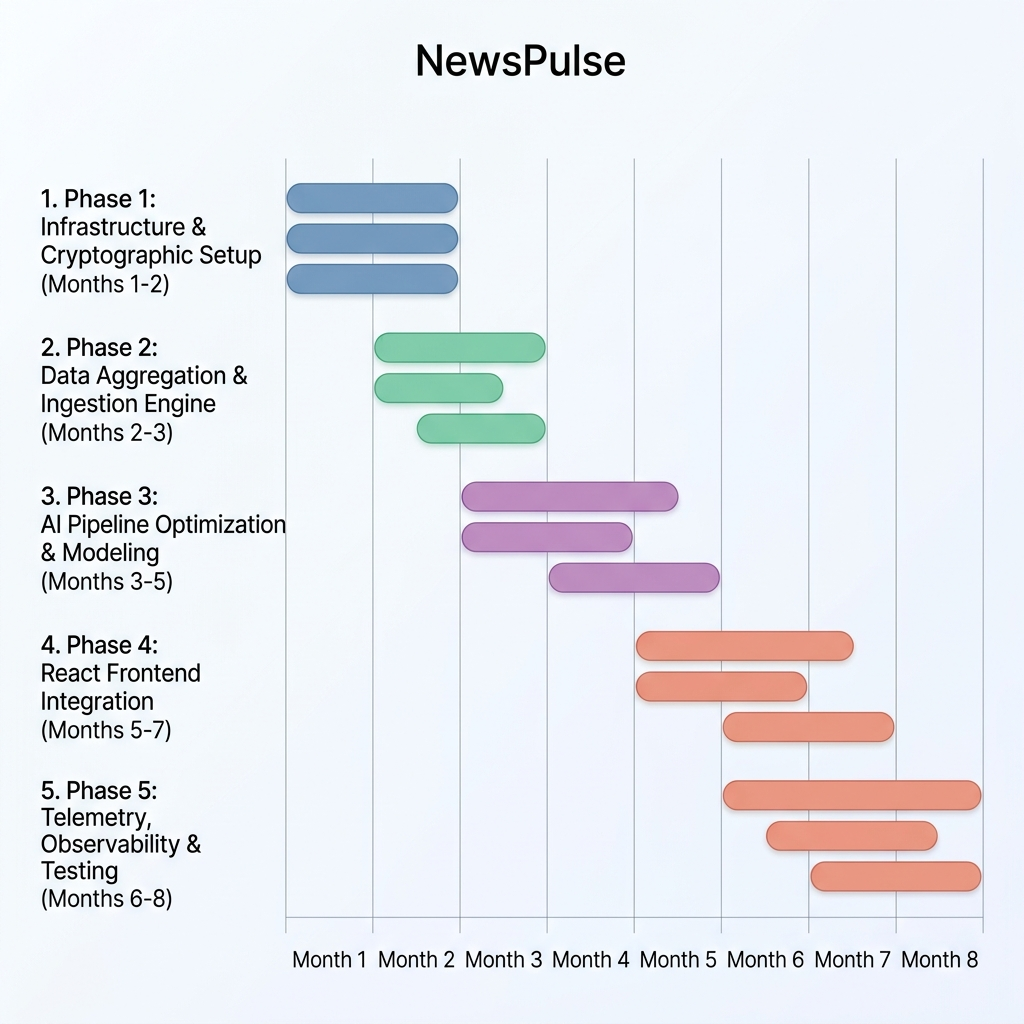
\includegraphics[width=\textwidth]{BS_FYP_Figs/gantt_chart.png}
    \caption{Project Implementation Gantt Chart}
    \label{fig:gantt_chart}
\end{figure}

\section{Report Outline}
The remainder of this document is structured into the following chapters:
Chapter 2 (Software Requirement Specifications) establishes the comprehensive functional and non-functional requirements of the system, detailing hardware/software boundaries, user characteristics, and structural constraints for localized deployment.
Chapter 3 (Use Case Analysis) provides a granular exploration of core system operations, presenting detailed actor behaviors, preconditions, execution flows, and exceptions for account actions and analytical pipelines.
Chapter 4 (System Design) documents the structural blueprints of the platform, including UML sequence diagrams, component configurations, centralized API gateway routing, and relational database schemas.
Chapter 5 (Implementation) details the core programming methodologies, explaining CPU-friendly transformer optimizations, PyTorch dynamic integer quantization, deterministic scraping heuristics, and hybrid cryptosystem integrations.
Chapter 6 (Business Plan) outlines the economic viability of the project, presenting target market demographics, monetization models, SWOT analysis, and operational cost projections.
Chapter 7 (Testing \& Evaluation) evaluates the platform's robustness under load, presenting functional validations, boundary testing outcomes, payload transit protection verifications, and real-time Prometheus telemetry.
Chapter 8 (Conclusion \& Future Work) summarizes the completed engineering milestones and technical contributions of the project, while presenting scalable paths for distributed crawling expansions.
